\chapter{Implementación}

	\section{Mapa caótico}
    
        En el artículo \cite{Sprott1993} y \cite{Fraga2021}
        \begin{equation}
            \begin{array}{ccl}
                x_{n+1} & = &  a_{1} + a_{2}x_{n} + a_{3}x_{n}^{2} + a_{4}x_{n}y_{n} + a_{5}y_{n} + a_{6}y_{n}^{2}\\
                y_{n+1} & = &  a_{7} + a_{8}x_{n} + a_{9}x_{n}^{2} + a_{10}x_{n}y_{n} + a_{11}y_{n} + a_{12}y_{n}^{2}
            \end{array}
        \end{equation}
        
        donde los parámetros $\{a_{1}, a_{2}, \ldots a_{12}\}$ pueden tomar diferentes valores, sin embargo para este trabajo se usaron los siguientes:


        \begin{equation}
            \begin{array}{ccl}
                x_{n+1} & = &  a_{1} + ( a_{2} + a_{3}x_{n} )x_{n} + a_{4}x_{n}y_{n} + ( a_{5} + a_{6}y_{n} )y_{n} \\
                y_{n+1} & = &  a_{7} + ( a_{8} + a_{9}x_{n} )x_{n} + a_{10}x_{n}y_{n} + ( a_{11} + a_{12}y_{n})y_{n}
            \end{array}
        \end{equation}

        \begin{equation}
             \begin{array}{lcl}
                M_{1} & = & \{ -0.6, -0.1, 1.1, 0.2, -0.8, 0.6, -0.7, 0.7, 0.7, 0.3, 0.6, 0.9 \}\\
                M_{2} & = & \{ -1.0, 0.9, 0.4, -0.2, -0.6, -0.5, 0.4, 0.7, 0.3, -0.5, 0.7, -0.8 \}\\
                M_{3} & = &  \{0.8, 1.0, -1.2, -1.0, 1.1, -0.9, 0.4, -0.4, -0.6, -0.2, -0.5, -0.7 \}\\
                M_{4} & = & \{-0.6, -0.4, -0.4, -0.8, 0.7, 0.3, -0.4, 0.4, 0.5, 0.5, 0.8, -0.1 \}
            \end{array}
        \end{equation}

        \begin{equation}
            \begin{array}{lcl}
                s_{n+1} = \{ x_{n+1} \text{ mod } 256, y_{n+1} \text{ mod } 256 \}
            \end{array}
        \end{equation}

        \begin{table}[htbp]
            \centering
            \caption{Exponentes de Lyapunov y dimensión fractal (tomados de \cite{Sprott1993}) de los mapas 2D usados.}
            \begin{tabular}{|l|l|l|}
                \hline
                \rowcolor[rgb]{ .682,  .667,  .667}Mapa  & Exponentes de Lyapunov & Dimensión fractal \\
                \hline
                1     & 0.12                   & 1.77   \\
                \hline
                2     & 0.14                   & 1.79   \\
                \hline
                3     & 0.15                   & 1.69   \\
                \hline
                4     & 0.13                   & 1.50   \\
                \hline
            \end{tabular}
        \end{table}

        \begin{table}[htbp]
            \centering
            \caption{Número de bits usados en la implementación de cada uno de los mapas con aritmética de punto fijo.}
            \begin{tabular}{|l|l|l|}
                \hline
                \rowcolor[rgb]{ .682,  .667,  .667}Mapa  & Bits parte entera & Bits parte fraccionaria \\
                \hline
                1     & 3                   & 60   \\
                \hline
                2     & 4                   & 59   \\
                \hline
                3     & 4                   & 59   \\
                \hline
                3     & 3                   & 60   \\
                \hline
            \end{tabular}
        \end{table}

        \begin{table}[htbp]
            \centering
            \caption{Rangos usados para la condición inicial para cada uno de los mapas.}
            \begin{tabular}{|l|l|}
                \hline
                \rowcolor[rgb]{ .682,  .667,  .667}Mapa  & Rango de valores para $x_{0}$ y $y_{0}$ \\
                \hline
                $M_{1}$  & $x_{0} \in [-0.5, \phantom{-} 0.5]$, $y_{0} \in [-0.5, \phantom{-}0.5]$ \\
                \hline
                $M_{2}$  & $x_{0} \in [-1.0, \phantom{-} 0.0]$, $y_{0} \in [\phantom{-}0.0, \phantom{-}1.0]$ \\
                \hline
                $M_{3}$  & $x_{0} \in [\phantom{-}0.0, \phantom{-} 1.0]$, $y_{0} \in [-0.6, \phantom{-}0.4]$ \\
                \hline
                $M_{4}$  & $x_{0} \in [-1.5, -0.5]$, $y_{0} \in [-0.5, \phantom{-}0.5]$ \\
                \hline
            \end{tabular}
        \end{table}

        \begin{figure}[hbtp]
            \caption{Diagrama de bloques del mapa caótico.}
            \centering
            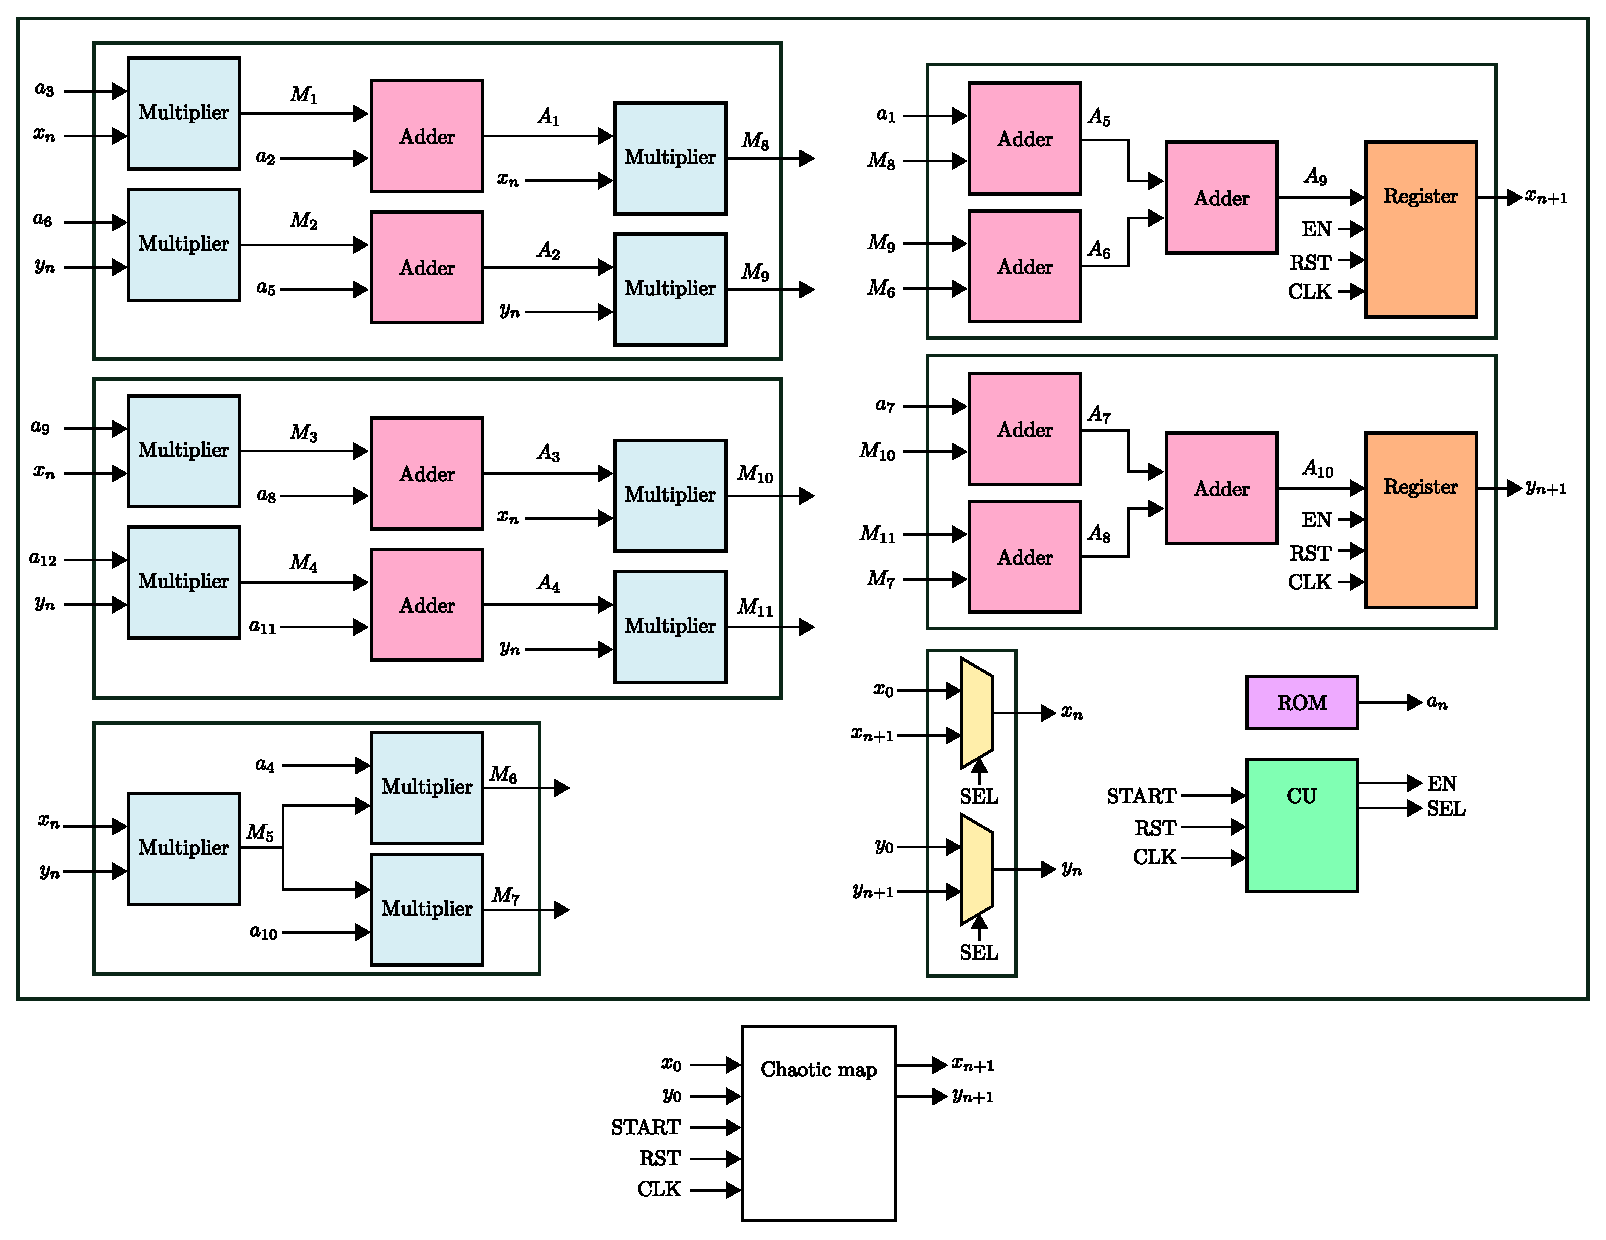
\includegraphics[width=0.9\linewidth]{B1_architecture}
            \label{fig:B1_architecture}
        \end{figure}

        \begin{figure}[hbtp]
            \caption{Máquina de estados de mapa caótico.}
            \centering
            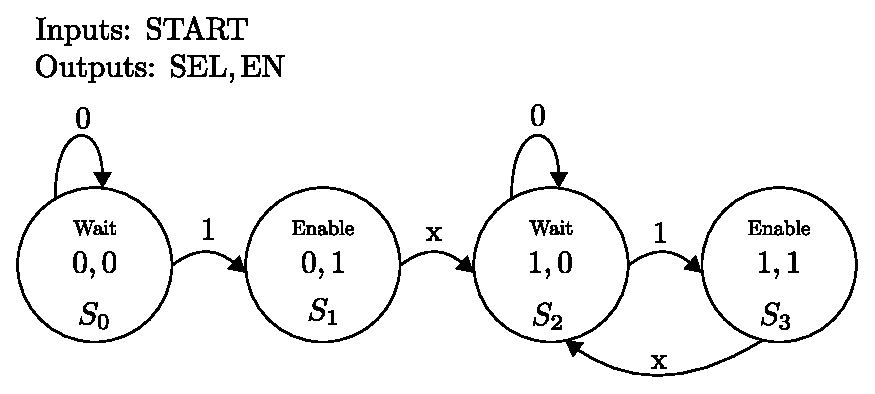
\includegraphics[width=0.6\linewidth]{B2_fsm_cm}
            \label{fig:B2_fsm_cm}
        \end{figure}

        \begin{figure}[hbtp]
            \caption{Simulación del mapa caótico en punto flotante.}
            \centering
            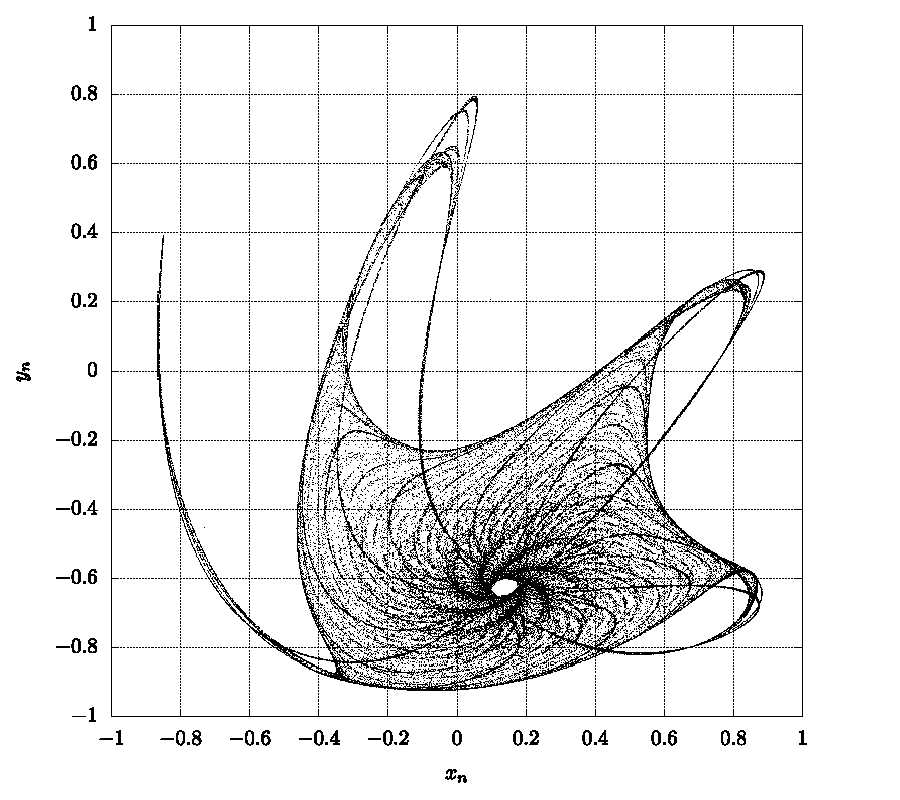
\includegraphics[width=0.8\linewidth]{B0_chaotic_map}
            \label{fig:B0_chaotic_map}
        \end{figure}

    \section{Single Constant Multiplier (SCM)}


    \section{Comunicación RS232}

        \begin{figure}[hbtp]
            \caption{Diagrama de bloques de transmisión RS232.}
            \centering
            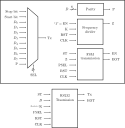
\includegraphics[width=0.6\linewidth]{C1_architecture_rs232}
            \label{fig:C1_architecture_rs232}
        \end{figure}

        \begin{figure}[hbtp]
            \caption{Máquina de estados para la transmisión RS232.}
            \centering
            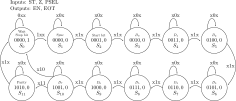
\includegraphics[width=0.8\linewidth]{C0_fsm_rs232}
            \label{fig:C0_fsm_rs232}
        \end{figure}	

    \section{Diseño de TRNG}

        \begin{figure}[hbtp]
            \caption{Diagrama de bloques de TRNG.}
            \centering
            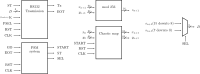
\includegraphics[width=0.9\linewidth]{D0_system}
            \label{fig:D0_system}
        \end{figure}

        \begin{figure}[hbtp]
            \caption{Máquina de estados de TRNG.}
            \centering
            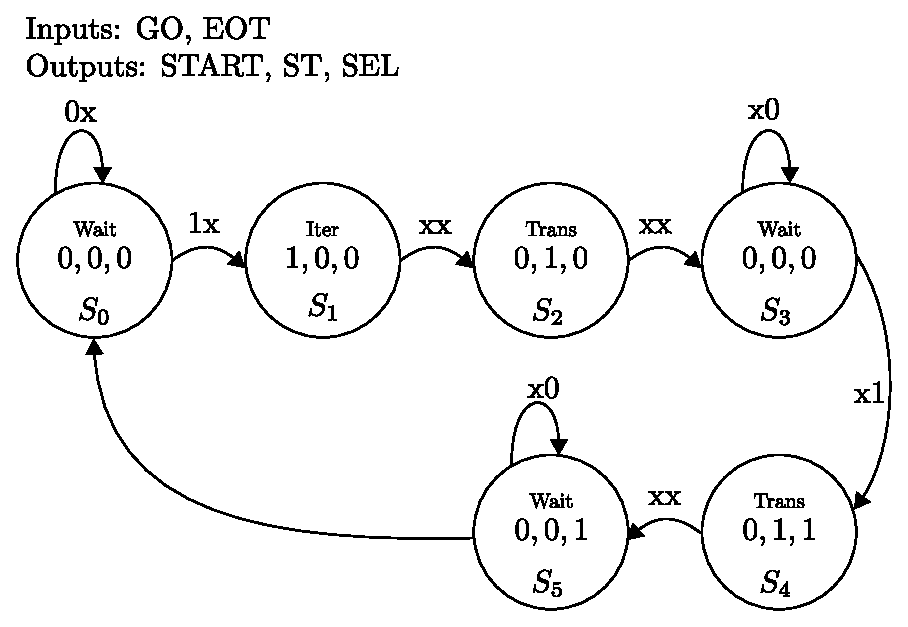
\includegraphics[width=0.7\linewidth]{D1_fsm_system}
            \label{fig:D1_fsm_system}
        \end{figure}

	\begin{comment}

	
\begin{table}[htbp]
  \centering
  \caption{Resumen de los resultados de implementación de las TRNGs}
\resizebox{0.5\linewidth}{!}{ 
    \begin{tabular}{lll}
   & Test name                 & Prop. \\
   \hline
1  & Frequency                 & 0.99  \\
2  & Block frequency           & 0.99  \\
3  & Runs                      & 1.00     \\
4  & Longest run               & 1.0     \\
5  & Rank                      & 0.98  \\
6  & DFT                       & 0.99  \\
7  & Non-overlapping templates & 1.00     \\
8  & Overlapping templates     & 0.99  \\
9  & Universal                 & 0.99  \\
10 & Linear complexity         & 0.99  \\
11 & Serial                    & 0.99  \\
12 & Approximate Entropy       & 0.99  \\
13 & Cumulative Sums           & 0.99  \\
14 & Random excursions         & 0.99  \\
15 & Random excursions variant & 1.00    
    \end{tabular}
}
  \label{tab:asdasd}
\end{table}


\newpage
	




	\end{comment}

